% Chapter3.tex
\chapter{\textsc{Cinco} Product Application}\label{ch:CP}

Having described the metalevel of the graphical modeling tool, we come now to the description of the model editor instantiated from it. The goal of this chapter is to explain the the appearance and behavior of the various model elements. First, we give a succinct definition of a graphical DSL, then illustrate the fundamental building blocks of our documentation model and by presenting at the same time the \textsc{Cinco} product application. Later on, we demonstrate the use of these graphical elements to specify the important configuration of the website we want to document. At the end, we show how using the editor built-in generator, a project structure, that constitute the target application, is generated.

\section{Graphical DSL}\label{sec:gDSL}

Under \acrfullpl{dsl} we understand a languages tailored to describe or solve problems in a specific computational domain. They represent the core concept of most state-of-the-art software development paradigms~\cite{perez-et_al}. As stated in~\cite{Naujokat2018}, one of their great advantage is that they permit domain experts with no programming experience to design application by means of graphical components, whose behavior and semantic have been or will be programed by developers with coding experience. The graphical aspect --- meaning that there is no use of textual grammar to construct a model --- adds an abstraction layer that eliminates a bit further the necessity of mastering the syntax of the underlying DSL, as well as the \acrshortpl{api} intertwining the metamodel elements.

In our case, the graphical model is composed of node elements, which have been applied different appearances to, in order to resemble to some extent the corresponding web elements they represent. The purpose behind this approximated replication is not to recreate all possible web elements, but to give the developer a sense of control over the interactable UI elements. With those elements at hand, the designer can simply model a user action by arranging node elements following the sequence it would require in the web application. This graphical language is in such way domain specific, that it is tailored for modeling sequences in a web application driven inside a web browser; modeling a documentation for a desktop application for example is not possible.

\section{Graph Editor}\label{sec:graphEditor}

The editor is mainly composed of the canvas in the middle of the working environment (1), where the developer can drag and drop model elements from the palette located on the right-hand side (2). Herein, elements are grouped in a single category; this is achieved using the \lstinline[language=MGL]{@palette("category name")} annotation in the~.mgl meta-specification (see line~\ref{line:paletteAnnotation} in listing~\ref{docMGL}). On the left-hand side we have the project explorer showing the current project structure (3). The main model files have the extensions .doc and .feat, where the latter is the entry point of the documentation application. By hovering over a model element, an arrow symbol appears, allowing the developer to similarly drag and drop connecting edges from the source to the target element. 

\begin{figure}[h]
    \centering
    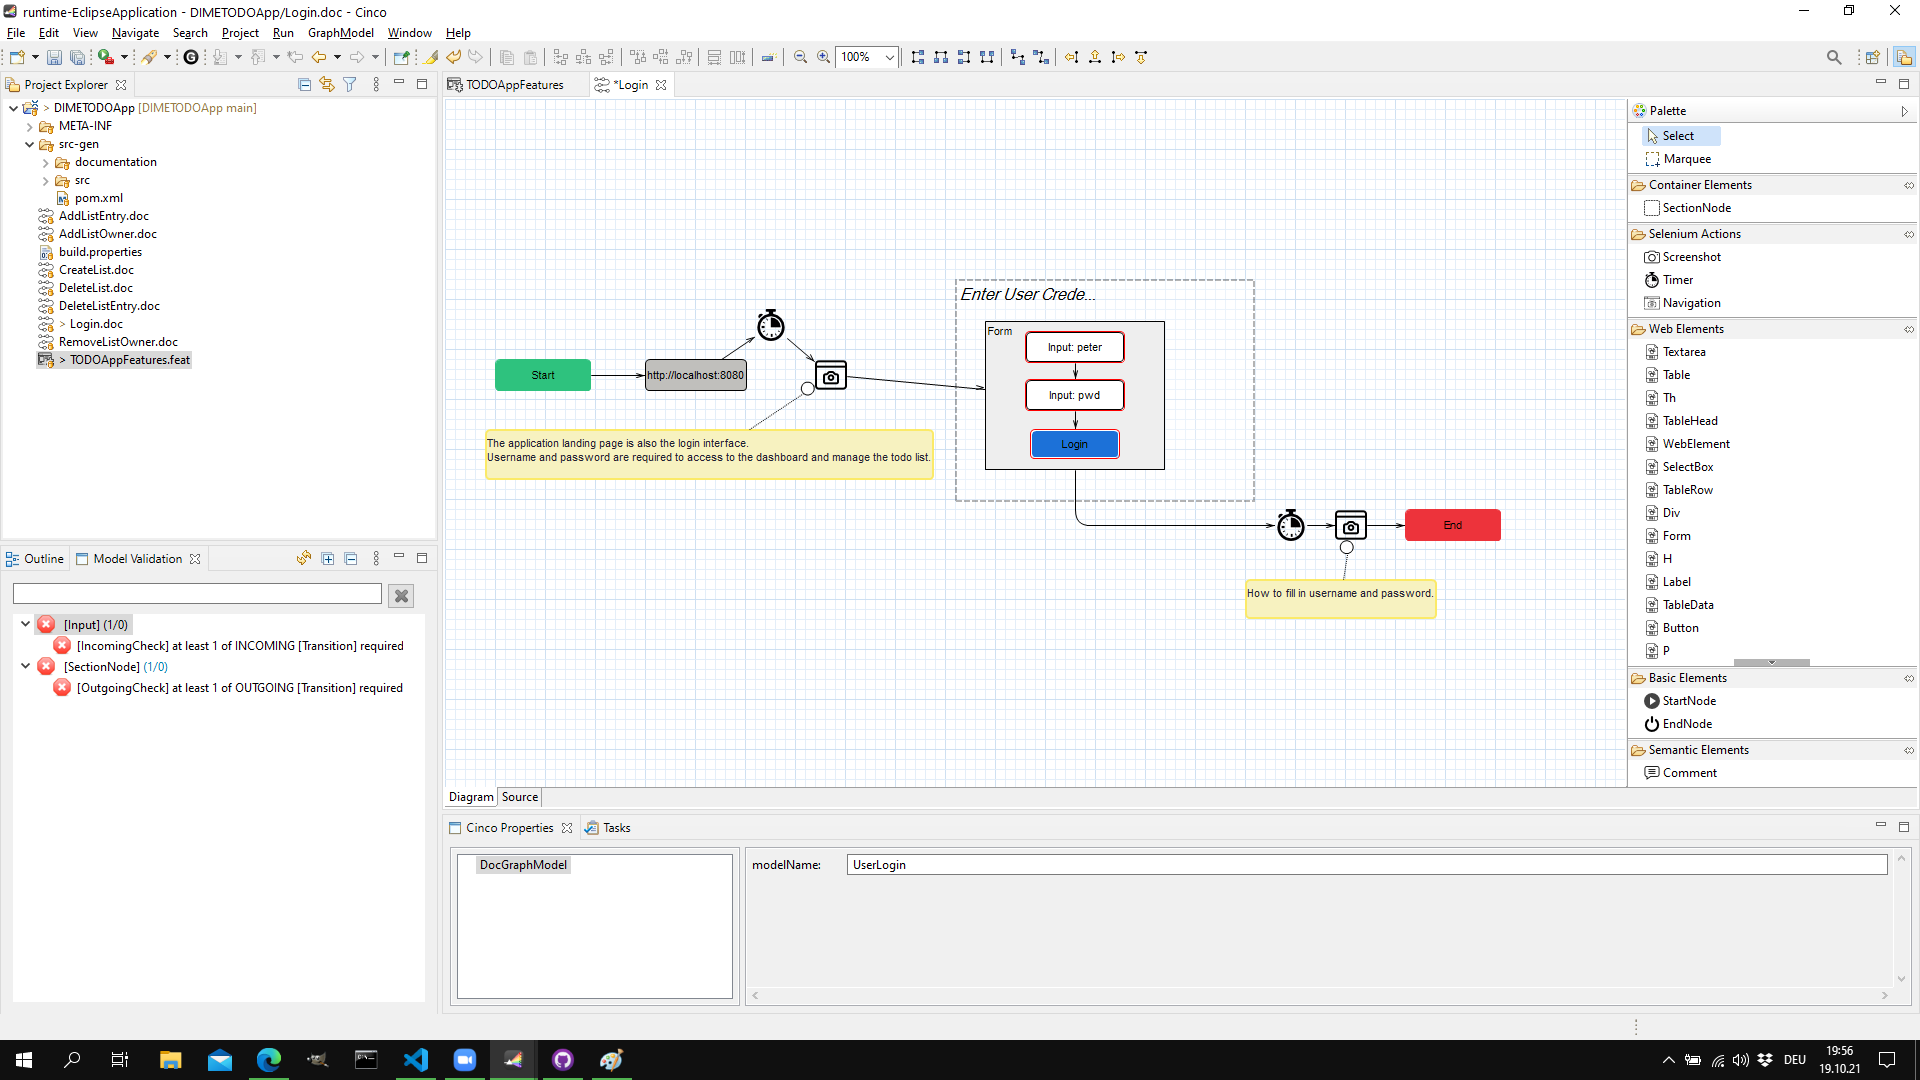
\includegraphics[width=\textwidth]{DocGraphModelChecks.png}
    \caption{\textsc{Cinco} Product Application - Graph model editor}\label{fig:graphDSL}
\end{figure}

All diagrams that are open in the editor are checked in the background for compliance with the requirements described on the metalevel using the \lstinline[language=MGL]{@mcam("check")} and shown in the Model Checking view right beneath the project explorer (4). There's also the \textsc{Cinco} property view (5) that displays the attributes and values of any selected element in the editor. This is where the developer can modify those values if the attribute field allows it.

The example model shown in Figure~\ref{fig:loginSeq} illustrate the sequence an end-user would eventually undergo to login to the web application. Showing the web elements that will be interacted with and how combined into a logical sequence, they form a user workflow. The sequence begins with the start node then comes a navigation node with the link attribute pointing to \lstinline{http://localhost:8080}, the landing page of our TODO Web App in development.Next, the timer node waits explicitly for an amount of second the designer specified in the property view. The palette view presents a list of all the available graph model elements (see table~\ref{tab:listOfElements}). Since we specified two different \acrshortpl{mgl}, the list in the DocGraphModel differs from the one in the FeatureGraphModel. For instance, the DocGraphModel has a whole category for web elements specified, because the user action sequence is modeled using common UI elements of the web interface. On the other hand, the FeatureGraphModel is specially there to provide some start configuration (e.g. the path to the webdriver executable to be used), meaning that it regroups all the features modeled in every DocGraphModel, builds up both project structures mentioned before and triggers the code generation for every single one of them.

\begin{figure}[h]
    \centering
    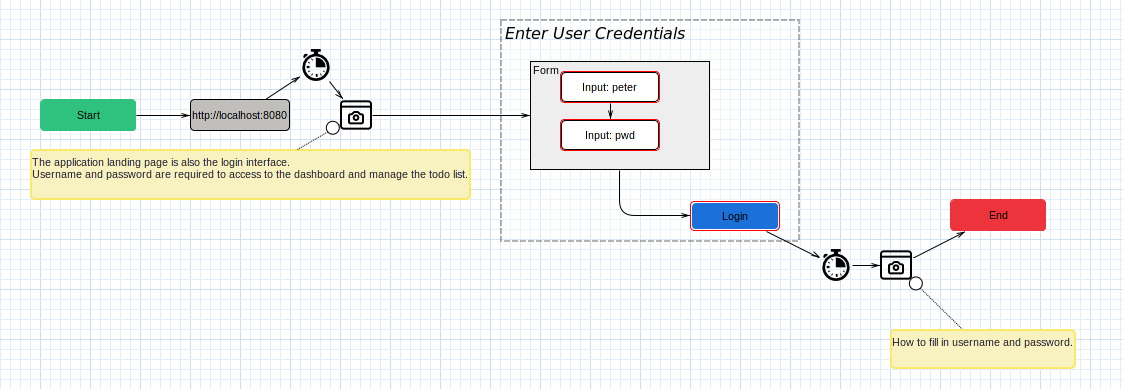
\includegraphics[width=\textwidth]{LoginSequence.png}
    \caption{Example of a user workflow: here the login sequence}
    \label{fig:loginSeq}
\end{figure}

\section{Feature Model Elements}\label{sec:FeatModElem}

The feature graph model is the application starting point. Here, the developer groups all the feature that needs to be documented in feature containers. Figure~\ref{fig:featGraph} depicts a portion of the features modeled for our TODO application. The important abilities of the web application are regrouped here: the ability to login, to create a new list, add a task to that list or remove it and lastly delete the whole list. Nonetheless, our TODO application offers the possibility to also add a new list owner, which already exist in the system as regular user. Those features are not represented to reasonable size of the image where the elements are clearly seen. On the top left-hand corner you can see an property container holding the webdriver property, whose value is set to \lstinline[language=MGL]{FIREFOX}. This value will be assigned to the Selenium webdriver variable in the Java class. Remember that the executable file for the chosen webdriver muss already exist somewhere in file system and the path to it has to been specified here in the property view.

\begin{figure}[H]
    \centering
    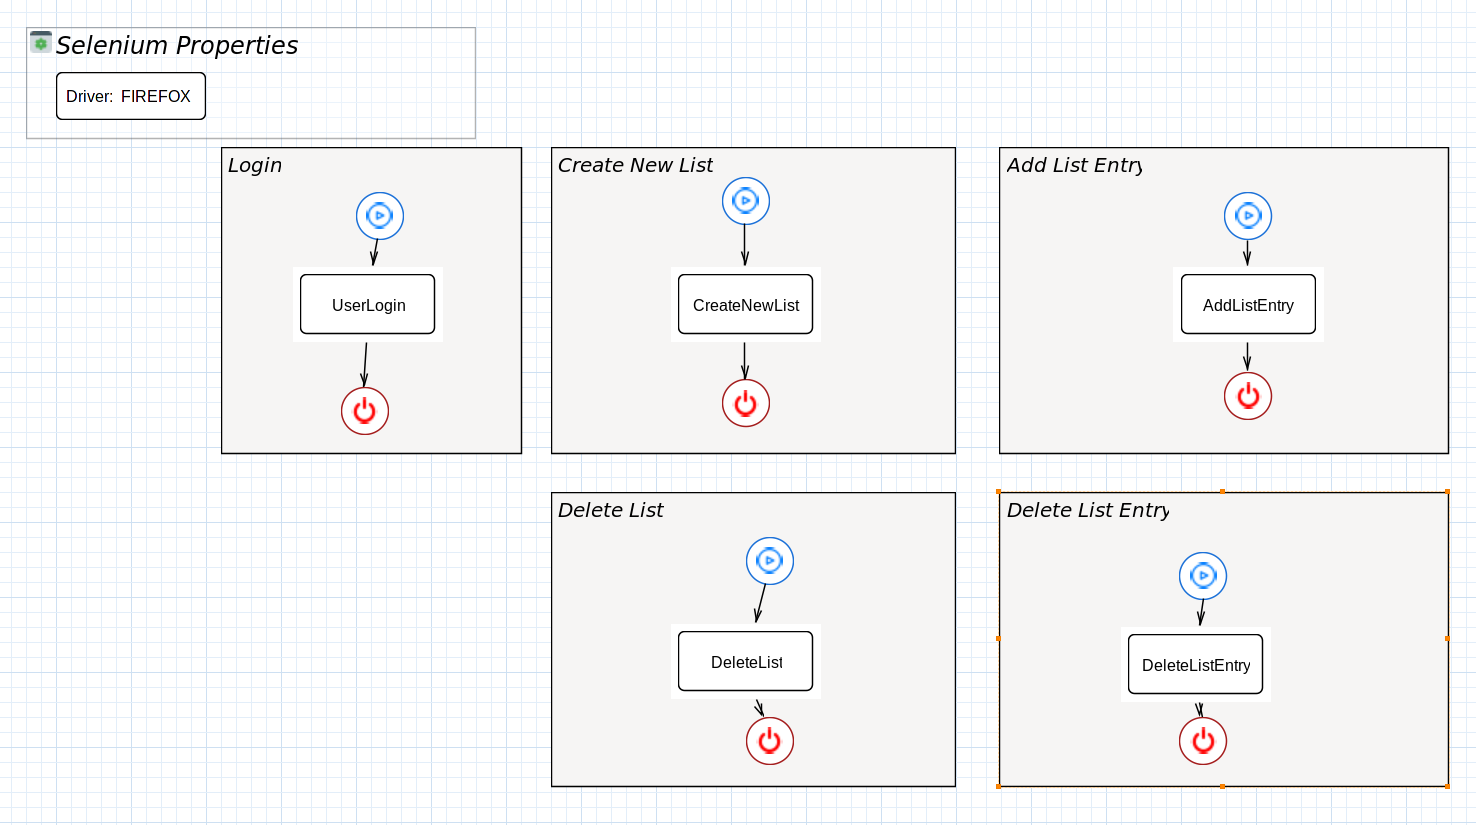
\includegraphics[width=\textwidth]{FeatureGraphModel2.png}
    \caption{\textsc{Cinco} product - Feature Graph Model with Feature Containers}
    \label{fig:featGraph}
\end{figure}

Even though we represented the features in logical order, they still are independent from one another and will be generate in the same manner. This separation does not exclude reusability, since it is possible to integrate a whole DocGraphModel inside another one.

\section{User Action Model Elements}\label{sec:DocModElem}


\section{Generation Process}\label{sec:GenProcess}

As mentioned before, the prominent feature of \textsc{Cinco} is the generate button. This allows the developer, after the modeled has been laid out without errors, to generate the a fully realized Selenium-Java application, which is going to execute the user sequence model just created. Figure~\ref{fig:genButton} shows where the generate button is located.

\begin{figure}[H]
    \centering
    
\includegraphics[width=\textwidth]{GenerateButtonHighlighted.png}
    \caption{\textsc{Cinco} product - generator button}
    \label{fig:genButton}
\end{figure}
